\chapter[API]{API}

\section{Visão Geral}
Para integração entre o Facebook e outros aplicativos externos é necessário o uso de uma API, a disponibilizada pela rede social em questão é a Graph. Ela é usada para que aplicativos externos possam realizar as requisições e envio de dados, possibilitando consulta e gerência dos dados presentes na rede social. 

Um sistema de permissões é utilizando na Graph API para controle de acesso e controle de publicação e de edição de informações. Assim, para que alguma modificação no modulo administrador possa ser efetivada, é necessário possuir as permissões adequadas. As permissões necessárias para o completo uso do aplicativo foram configuradas durante o desenvolvimento do SID e serão solicitadas durante o processo de login do usuário que tentar acessar.

As permissões descrevem quais as possíveis ações podem ser feitas em cooperação com a Graph API, elas determinam quais tipos de dados pode-se gerenciar e quais as possíveis respostas o sistema pode retornar.

A estrutura da Graph, segue a de um grafo, onde possui nós, arestas e atributos (campos). Nós são objetos individuais, cada nova página, usuário, comentário ou foto criada no Facebook é considerado um nó \cite{facebook2018b}. Usando o nó é possível se obter as bordas, no caso fotos de uma página ou comentários em uma foto. A página do SID é um nó, usando o ID único dela é possível criar novas publicações que serão vinculadas a esse nó, essas novas publicaçãos serão formados do ID da página acrescidos de um ID único da foto, esse ID único da foto é considerado um outro novo nó. Usando ele é possível recuperar comentários e \textit{likes} \cite{facebook2018b}.

A autenticação no módulo administrador é feita usando um usuário cadastrado no Facebook e registrado no banco de dados do SID. O uso de um usuário vinculado a rede social se torna necessário pois existe a necessidade da página apresentar qual o perfil está realizando a ação, além da necessidade de moderação dos comentários que serão exibidos. 

Para autenticação e efetivação de todas as requisições feitas pelo aplicativo para o Facebook, seja ela para requisitar informações das publicações ou realizar uma nova publicação, é usando um \textit{token} de acesso, que é obtido após a efetivação de login do usuário com o Facebook. O \textit{token} é uma cadeia de caracteres que identifica um usuário, aplicativo ou página, identificando a sessão. Em cada nova requisição a rede social, o \textit{token} será usado, se autorizado, a aplicação poderá enviar requisições HTTP usando seus identificadores únicos, recebendo a respectiva resposta.

\section{Elementos Usados}
Para publicação no perfil pessoal, a Graph API requisita duas permissões, sendo a “email”, onde é requisitado o acesso ao endereço de email do usuário para que seja possível a autenticação do SID com o Facebook e a “publish\underline{{ }}actions”, onde fornece acesso a realização de publicações em nome da pessoa que está usando o aplicativo \cite{facebook2018a}.

Como o SID será usado em uma página e não em um perfil pessoal, duas novas autenticações se tornaram necessárias, sendo a “manage\underline{{ }}pages”, usada para recuperar as permissões de acesso a pagina e a “publish\underline{{ }}pages”, usada parar permitir que aplicativos publiquem na página \cite{facebook2018a}.

Usando o identificador único da foto é possível recuperar informações da borda, que são informações como a URL, comentários e curtidas. Esse recurso é utilizado para recuperar o endereço da publicação, os comentários e curtidas que serão apresentados respectivamente nos campos destinados ao QRCode e na coluna de comentários do módulo cliente.

Na criação de uma nova publicação, usando o SID, são passados para a Graph API dois parâmetros para inserção, o primeiro deles é “messagem”, onde será passado o texto que será exibido na publicação e o outro é “source”, onde será passado a imagem para ser exibida juntamente com o texto. Para envio de imagem para a rede social, é necessário passar a imagem como paramento do método “fileToUpload”. 

Alguns dos elementos que são solicitados pela aplicação na criação de uma nova publicação, são omitidos para o Facebook, pois esses dados serão usados apenas para serem armazenados no banco. Os elementos omitidos são os campos data de inicio, a data de termino e a legenda. 

------------------ CONTINUA  P48-------------------

\section{Integração}
Qualquer divulgação inserida na pagina do SID no Facebook utiliza-se do nó “photo”, ou seja, a divulgação que o SID repassa à Graph API contém a mesma estrutura de uma imagem postada por um usuário convencional desta rede social. 

A Figura \ref{fig:imgadministrador1} mostra todos os campos necessários para envio, isso é, como é estruturada a divulgação que será enviada ao perfil do SID no Facebook através da integração com a Graph API. Entre os campos estão: 
\begin{enumerate}[label=\Roman*)]
	\item O campo ``imagem''(\textit{source}), é a foto que irá ser exibida no Facebook e no módulo cliente.
	\item O campo ``texto''(\textit{messagem}), recebe o texto que irá ser exibido juntamente com a publicação.
\end{enumerate}

Todos os campos tem preenchimento obrigatório, entretanto, somente os dois citados anteriormente são enviados ao Facebook. Os outros campos não são enviados a rede social, ficam armazenados apenas no banco de dados, são eles:
\begin{enumerate}[label=\Roman*)]
	\item O campo legenda, que é um resumo do texto que será exibido no módulo cliente.
	\item O campo data de inicio e data de término, é a data em que a publicação começará e deixará de ser exibida no modulo cliente.
\end{enumerate}

Com as informações que são enviadas usando a Graph, é feito a chamada do método "post", nessa chamada é colocada todas as informações necessárias para que seja feito uma nova publicação no Facebook, com isso, ele faz a criação de um novo objeto ou seja, um novo nó. Caso alguma das transações não sejam efetivadas, será retornado a mensagem de erro, assim como a mensagem de sucesso, caso não ocorra nenhum erro.

------------------ CONTINUA  P49-------------------

----------- COLOCAR FOTO DA PUBLICAÇÃO DO FACEBOOK. -----------

 \begin{figure}[H]
\centering
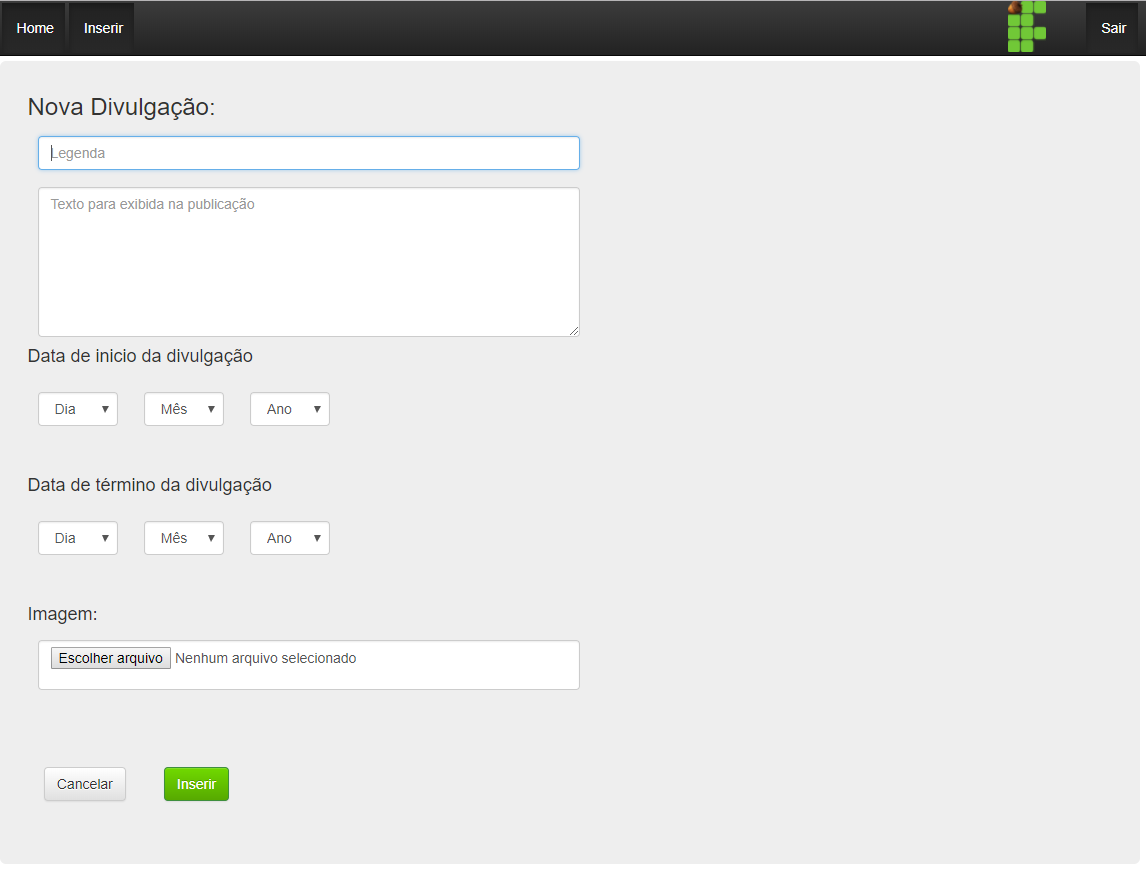
\includegraphics[scale=0.6]{figuras/administrador1}
\caption{Divulgação enviada a pagina do SID}
\label{fig:imgadministrador1}
\end{figure}